\documentclass[a4paper,kulak]{kulakarticle}

\usepackage[utf8]{inputenc}
\usepackage[dutch]{babel}
\usepackage{pdfpages}


\date{\today}
\address{
	Bachelor in de fysica\\
	Bachelor in de informatica\\
	Bachelor in de wiskunde\\
	Ingenieurswetenschappen}
\title{BDA App}
\author{Marthe B\"{o}ting\\
	Robin Bruneel\\
	Toon Ingelaere}

\begin{document}
	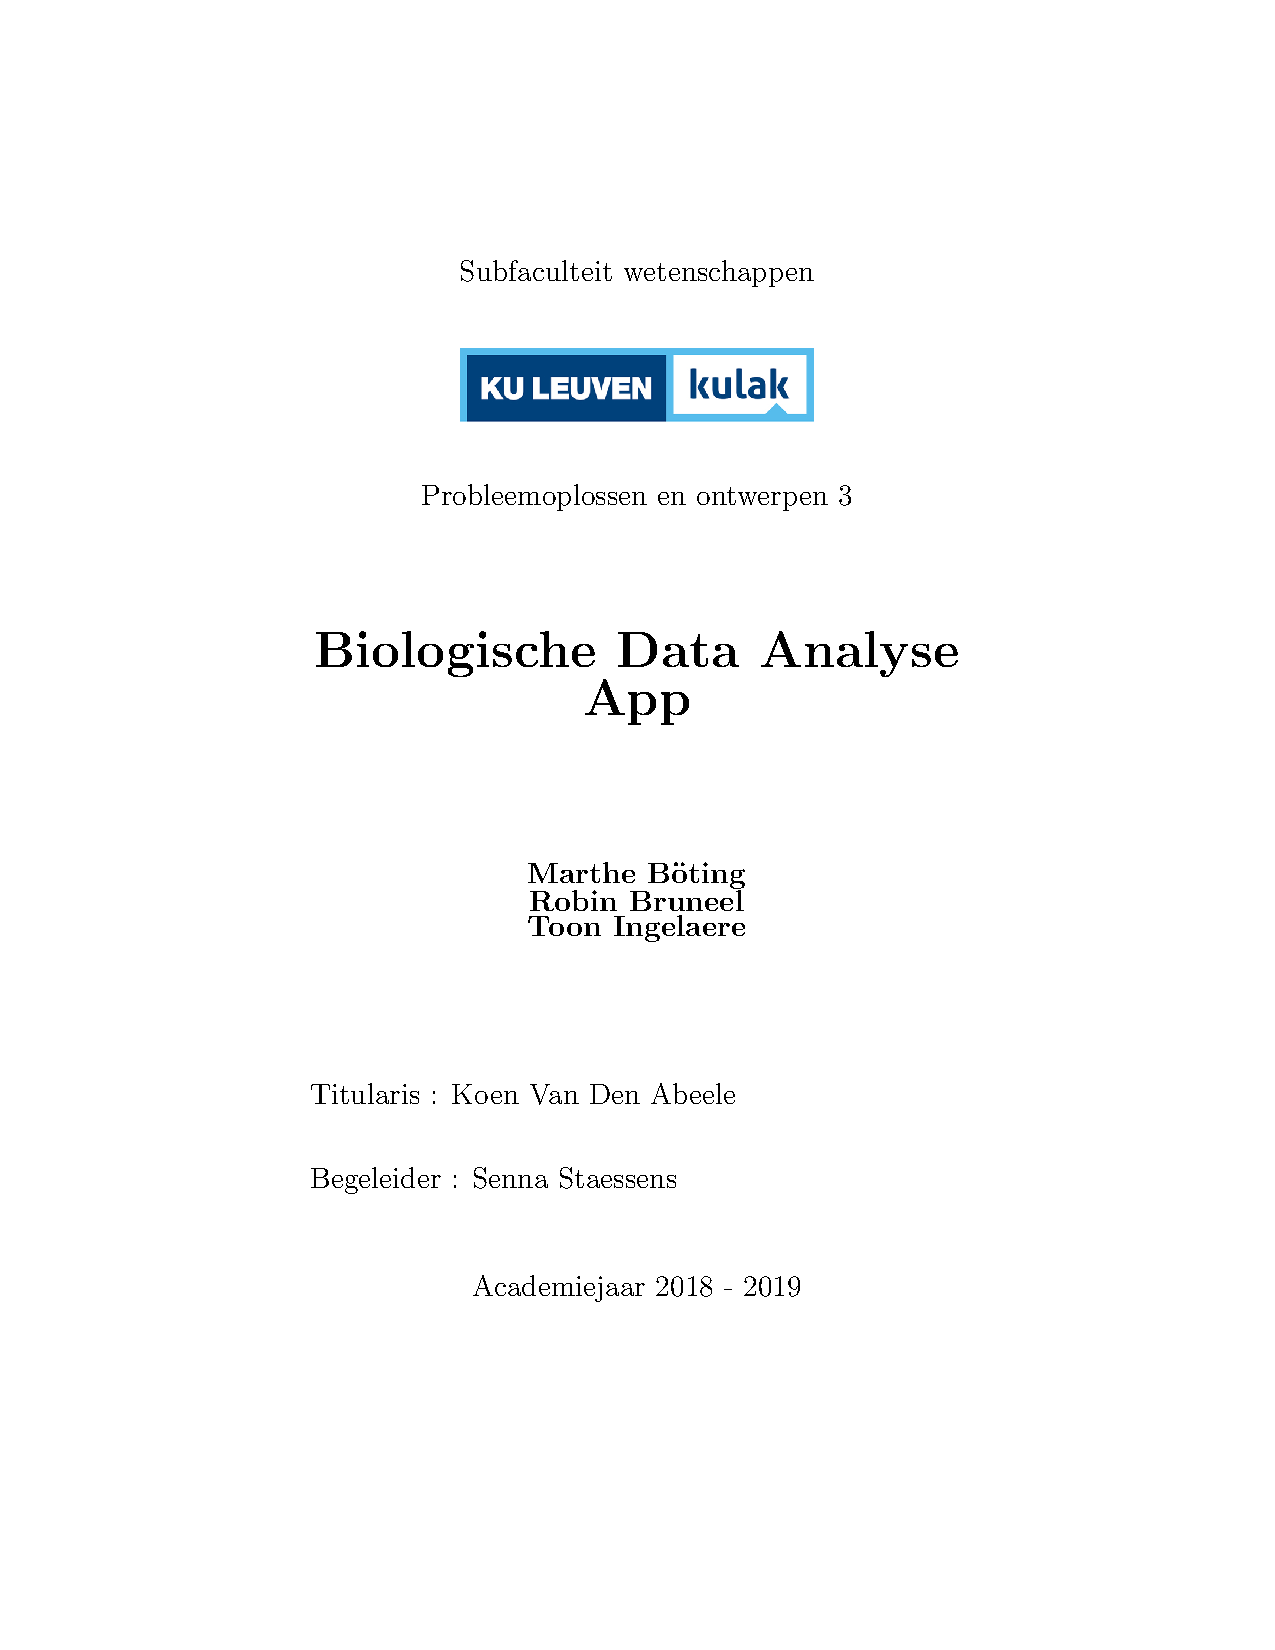
\includepdf{voorblad}
	\newpage
	\maketitle
	
	\section*{Inleiding}	
		Als gevolg van een bloedklonter in een hersenbloedvat ontstaat een ischemische beroerte. Deze klonter moet men zo snel mogelijk verwijderen dit kan met behulp van een geneesmiddel die de klonter oplost of door middel van mechanische verwijdering. Door deze mechanische verwijdering kan men de bloedklonter verder analyseren in het labo om een duidelijker beeld te krijgen.
		\newline
		Vandaag de dag verliest men zeer veel tijd aan het verwerken van de bloedklonters. Er is ons dan ook gevraagd om een app te ontwikkelen die de analyse van de foto’s volledig automatisch kan uitvoeren.
		\newline
		In dit verslag gaan we eerst in op wat de klant specifiek van ons verwacht en aan welke specificaties ons ontwerp moet voldoen. Hierna gaan we ons design bespreken en toelichten. Verder bespreken we ook onze voorlopige resultaten. Ten slotte wordt er nog een blik geworpen naar de vakken uit eerste 3 semesters die ons hierbij geholpen hebben.
	
	\newpage	
	\tableofcontents

	\section{Sectie-titel}	
		Tekst.
	
	\section*{Besluit}	
		Afsluitende tekst

\end{document}
